\section{Introduction}

LLMs have succeeded in various tasks, demonstrating impressive capabilities in generating human-like text and solving complex problems. However, their ability to accurately assess uncertainty in their predictions remains a significant challenge~\cite{kadavath2022language}. 
This gap between a model's confidence and its actual correctness, often called the confidence gap \cite{chhikara2025mindconfidencegapoverconfidence}, poses critical risks, particularly in high-stakes applications where overconfidence in incorrect answers leads to severe consequences: in domains such as health, law~\cite{Dahl_2024}, education, or economics an LLM's overestimation of its accuracy could result in harmful decisions or misinformation. 
Understanding and decreasing this confidence gap is therefore essential for ensuring the safe and reliable deployment of LLMs. 

Addressing this limitation has led to the development of numerous uncertainty estimation techniques. 
Most of them belong to one of two problem statements.
They either focus on binary classification or rely on rich signals from long, free-text responses~\cite{yang2024logulongformgenerationuncertainty}.
These methods often generalize poorly for concise multiple-choice questions.
\begin{figure}
    \centering
    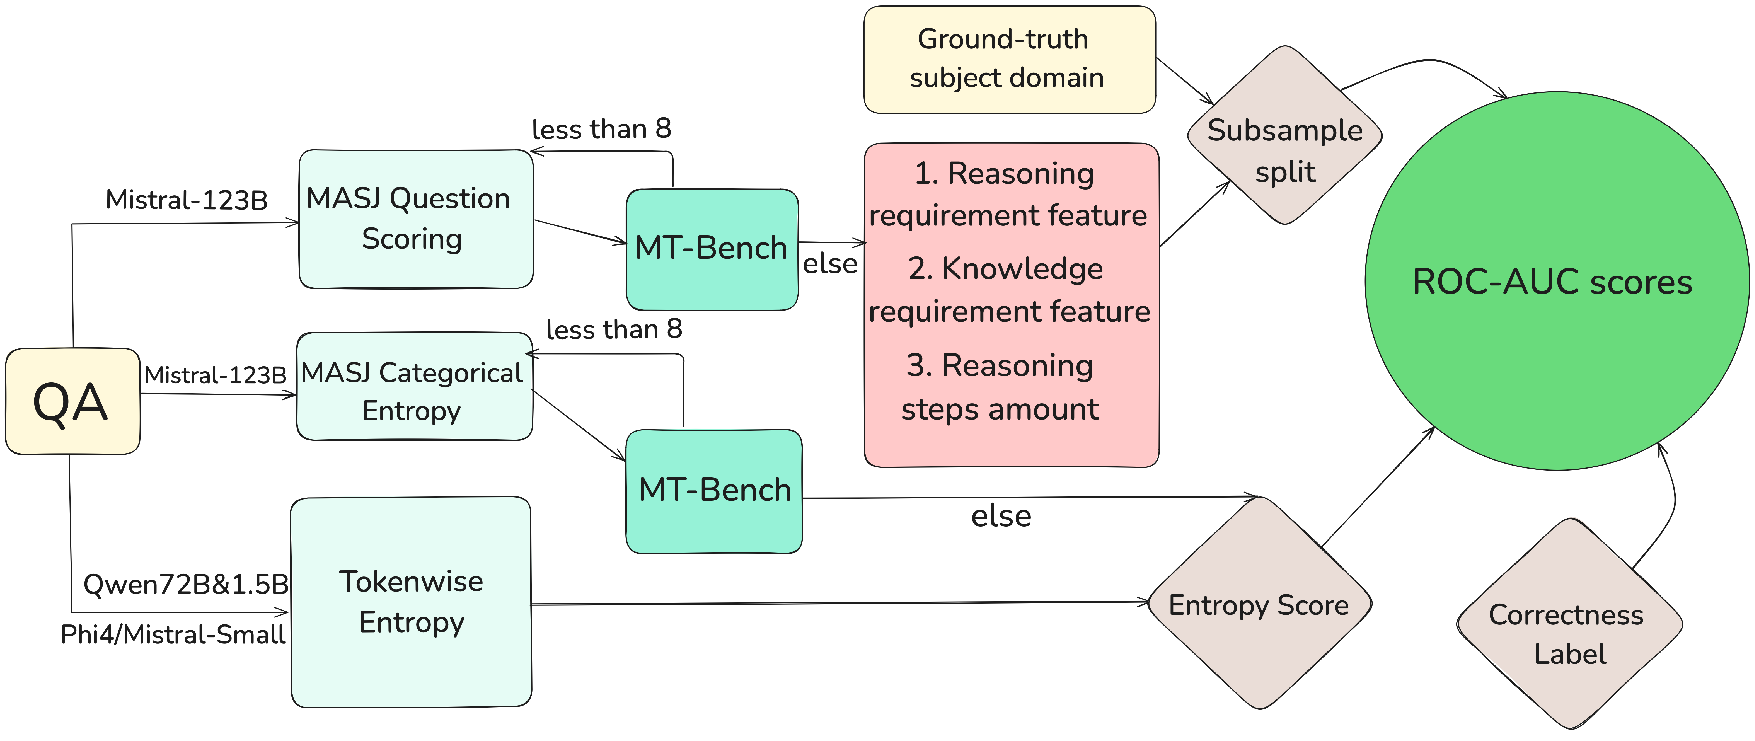
\includegraphics[width=1\linewidth]{images/pipeline_scheme.pdf}
    \caption{Question complexity evaluation pipeline. See more details in the methods section}
    \label{fig:difficult_questions_scheme}
\end{figure}

Moreover, existing methods tend to answer how good an overall confidence estimate is, ignoring why uncertainty appeared in a specific case. 
While classic decomposition of uncertainty to aleatoric (data) and epistemic (model)~\cite{hullermeier2021aleatoric} also holds for LLMs, the problem is challenging~\cite{huang2025survey}.
For example, the authors in~\cite{abbasi2025believe} consider only epistemic uncertainty.

To address these gaps, we propose a pipeline that enables detailed investigation of domain-specific or complexity-labeled datasets with multiple-choice answers. 
This framework allows us to explore how commonly used uncertainty estimation methods, particularly entropy-based approaches, perform under varying question topics and levels of required reasoning. 
We can also leverage an auxiliary LLM to generate labels for reasoning, knowledge requirements, and the number of reasoning steps. 
The introduction of the pipeline led to a more detailed investigation of datasets commonly used for benchmarking LLMs and their uncertainty estimates.
In more detail, our main contributions are the following:
\begin{itemize}
    \item We present a fully automated pipeline for evaluating uncertainty estimation approaches within the MMLU-Pro setting. It is presented in Figure~\ref{fig:difficult_questions_scheme} and allows datasets or tested methods to be varied. The associated work is available on Github\footnote{\url{https://github.com/LabARSS/question-complextiy-estimation}}.
    \item We propose using data uncertainty estimates based on token-wise entropy and model uncertainty estimates based on MASJ. Thus, our approach covers two main components of uncertainty estimation: data and model one, given that MMLU-Pro answers are typically short and provide limited information on model confidence.
    \item Within the developed pipeline, we consider different subsets of the MMLU-Pro dataset with splits by domain and reasoning requirement estimated via MASJ proposed in this work.
    \item Our experimental evidence that includes consideration of four models (Phi-4, Mistral-Small-24B-Instruct, Qwen-1.5 B, Qwen-72B) suggest that the entropy predicts well errors of an LLM if the amount of required reasoning is small. Moreover, its quality increases if the model size increases. Unlike MASJ provides much weaker results, being unable to identify error patterns. Further progress here would be possible with more reasoning steps during an uncertainty estimate with an entropy-based approach on top of it.
    \item We also observe that the existing dataset MMLU-Pro has internal biases with the complexity of the question, the same as in~\cite{gema2025mmlu}, and the required reasoning amount for them varies significantly depending on the topic. Thus, more advanced and less biased datasets are required for a fair measurement of the progress of LLMs. Additional human annotation of questions in a dataset could identify further gaps in LLMs' capabilities.
\end{itemize}